%#!pdfpLaTeX
%
% 北村研究室用卒業論文・特別論文のTeXテンプレートファイル
% 本ファイルは非公式であり,表紙とアブストに関しては下記で公開されているワードの
% テンプレートを利用して作成したものが公式であるので,表紙とアブストはPDFにして
% 差し替えること.
% https://www.kagawa-nct.ac.jp/EE/local/index.html (学内限定アクセス)
%
% 2020年1月17日 北村大地作成
%

%%%%%%%%%%%%%%%%%%%%%%%%%%% 論文情報 %%%%%%%%%%%%%%%%%%%%%%%%%%%
%%%%% テンプレート選択 %%%%%
%\documentclass[honka]{nitkcthesis}%卒論(本科5年)日本語用
%\documentclass[honka,english]{nitkcthesis}%卒論(本科5年)英語用
\documentclass[senkouka]{nitkcthesis}%特論(専攻科2年)日本語用
%\documentclass[senkouka,english]{nitkcthesis}%特論(専攻科2年)英語用

%%%%% タイトル %%%%%
\title{北村研究室用\\特別論文テンプレートファイル}
%\titlewidth{}% タイトル幅 (指定するときは単位つきで)

%%%%% 著者 %%%%%
\author{高専 太郎}
\eauthor{Taro Kosen}% Copyright表示で使われる

%%%%% 指導教員名 %%%%%
\supervisor{北村 大地 講師}% 1つ引数をとる (役職まで含めて書く)

%%%%% 提出年月 %%%%%
%\date{令和X年X月X日} % 和暦表示
\handin{2020}{2} % 西暦表示

%%%%% \usepackage等のプリアンブル宣言(macros.texに記載) %%%%%
\usepackage{bm}
\usepackage{amsmath, amssymb}
\usepackage[dvipdfmx]{color}
\usepackage[dvipdfmx]{graphicx}
\usepackage{tabularx}
\usepackage{booktabs}
\usepackage{multirow}
\usepackage{setspace}
\usepackage{amsthm}
\usepackage[caption=false]{subfig}
\usepackage[numbers,sort]{natbib}

\theoremstyle{definition}
\newtheorem{theo}{定理}[chapter]
\newtheorem{defi}{定義}[chapter]
\newtheorem{lemm}{補題}[chapter]
\renewcommand{\proofname}{\textbf{証明}}

%% definition
\newcommand{\J}{\mathrm{j}}
\newcommand{\diag}{\mathop{\mathrm{diag}}}

\newcommand{\mtr}[1]{#1^{\mathsf{T}}}
\newcommand{\ctr}[1]{#1^{\mathsf{H}}}
\newcommand{\inv}[1]{#1^{-1}}
\newcommand{\cinv}[1]{#1^{-\mathsf{H}}}
\newcommand{\tinv}[1]{#1^{-\mathsf{T}}}
\newcommand{\conj}[1]{#1^*}

\newcommand{\tbm}[1]{\tilde{\bm{#1}}}
\newcommand{\tsf}[1]{\tilde{\mathsf{#1}}}

\newcommand{\vw}{\bm{w}}
\newcommand{\mW}{\bm{W}}
\newcommand{\vwhat}{\widehat{\bm{w}}}
\newcommand{\mWhat}{\widehat{\bm{W}}}

\newcommand{\hhat}{\widehat{h}}
\newcommand{\rhat}{\widehat{r}}

\newcommand{\argmax}{\mathop{\mathrm{arg~max}}\limits}
\newcommand{\argmin}{\mathop{\mathrm{arg~min}}\limits}

\renewcommand{\Re}{\mathop{\mathrm{Re}}}
\renewcommand{\Im}{\mathop{\mathrm{Im}}}

\newcommand{\unit}[1]{~\mathrm{#1}}
\newcommand{\Unit}[1]{~\mathrm{\left[#1\right]}}

\renewcommand{\qedsymbol}{$\blacksquare$}

\bibliographystyle{bibstyle}

\makeatletter
\def\bstctlcite{\@ifnextchar[{\@bstctlcite}{\@bstctlcite[@auxout]}}
\def\@bstctlcite[#1]#2{\@bsphack
\@for\@citeb:=#2\do{%
\edef\@citeb{\expandafter\@firstofone\@citeb}%
\if@filesw\immediate\write\csname #1\endcsname{\string\citation{\@citeb}}\fi}%
\@esphack}
\makeatother


\renewcommand{\figurename}{Fig.} % 図中の文字や図キャプションを日本語で書く場合はこの行をコメントアウト(原則英語とする)
\renewcommand{\tablename}{Table} % 表中の文字や表キャプションを日本語で書く場合はこの行をコメントアウト(原則英語とする)

\begin{document}
\bstctlcite{IEEEexample:BSTcontrol} % BibTeXのIEEEtranで同一著者の横線表示を防止

\maketitle% タイトル生成

%%%%%%%%%%%%%%%%%%%%%%%%%%% 前文 %%%%%%%%%%%%%%%%%%%%%%%%%%%
\frontmatter

%%%%% English title %%%%%
\etitle{Template File of Graduate Thesis Produced Only for Kitamura Laboratory}

%%%%% Abstract %%%%%
\begin{eabstract} % これ単体で複数ページにまたがる場合はエラーが出るので注意,アブスト内で改段落は禁止
  English abstract goes here. English abstract goes here. English abstract goes here. English abstract goes here.
  English abstract goes here. English abstract goes here. English abstract goes here. English abstract goes here.
  English abstract goes here. English abstract goes here. English abstract goes here. English abstract goes here.
  English abstract goes here. English abstract goes here. English abstract goes here. English abstract goes here.
  English abstract goes here. English abstract goes here. English abstract goes here. English abstract goes here.
  English abstract goes here. English abstract goes here. English abstract goes here. English abstract goes here.
  English abstract goes here. English abstract goes here. English abstract goes here. English abstract goes here.
  English abstract goes here. English abstract goes here. English abstract goes here. English abstract goes here.
\end{eabstract}

%%%%% 概要 %%%%%
\begin{abstract} % これ単体で複数ページにまたがる場合はエラーが出るので注意,アブスト内で改段落は禁止
  日本語の概要をここに記述.日本語の概要をここに記述.日本語の概要をここに記述.日本語の概要をここに記述.
  日本語の概要をここに記述.日本語の概要をここに記述.日本語の概要をここに記述.日本語の概要をここに記述.
  日本語の概要をここに記述.日本語の概要をここに記述.日本語の概要をここに記述.日本語の概要をここに記述.
  日本語の概要をここに記述.日本語の概要をここに記述.日本語の概要をここに記述.日本語の概要をここに記述.
  日本語の概要をここに記述.日本語の概要をここに記述.日本語の概要をここに記述.日本語の概要をここに記述.
  日本語の概要をここに記述.日本語の概要をここに記述.日本語の概要をここに記述.日本語の概要をここに記述.
  日本語の概要をここに記述.日本語の概要をここに記述.日本語の概要をここに記述.日本語の概要をここに記述.
  日本語の概要をここに記述.日本語の概要をここに記述.日本語の概要をここに記述.日本語の概要をここに記述.
  日本語の概要をここに記述.日本語の概要をここに記述.日本語の概要をここに記述.日本語の概要をここに記述.
\end{abstract}

%%%%% 目次 %%%%%
% \setcounter{tocdepth}{3} \tableofcontents % ページ番号を削除しない目次
%----- ページ番号を削除した目次 -----%
{\makeatletter
\let\ps@jpl@in\ps@empty
\makeatother
\pagestyle{empty}
\setcounter{tocdepth}{3}
\tableofcontents
\clearpage}
%---------------------------------%

%%%%%%%%%%%%%%%%%%%%%%%%%%% 本文 %%%%%%%%%%%%%%%%%%%%%%%%%%%
\mainmatter

%%%%% 第1章 %%%%%
\chapter{緒言}
\label{chap:intro}

%----------------------------------------------
\section{本論文の背景}
%----------------------------------------------
本論文の背景をここに記載.本論文の背景をここに記載.本論文の背景をここに記載.本論文の背景をここに記載.
本論文の背景をここに記載.本論文の背景をここに記載.本論文の背景をここに記載.本論文の背景をここに記載.
本論文の背景をここに記載.本論文の背景をここに記載.本論文の背景をここに記載.本論文の背景をここに記載.
本論文の背景をここに記載.本論文の背景をここに記載.本論文の背景をここに記載.本論文の背景をここに記載.
本論文の背景をここに記載.本論文の背景をここに記載.本論文の背景をここに記載.本論文の背景をここに記載.
本論文の背景をここに記載.本論文の背景をここに記載.本論文の背景をここに記載.本論文の背景をここに記載.
本論文の背景をここに記載.本論文の背景をここに記載.本論文の背景をここに記載.本論文の背景をここに記載.
本論文の背景をここに記載.本論文の背景をここに記載.本論文の背景をここに記載.本論文の背景をここに記載.
本論文の背景をここに記載.本論文の背景をここに記載.本論文の背景をここに記載.本論文の背景をここに記載.
本論文の背景をここに記載.本論文の背景をここに記載.本論文の背景をここに記載.本論文の背景をここに記載.
本論文の背景をここに記載.本論文の背景をここに記載.本論文の背景をここに記載.本論文の背景をここに記載.
本論文の背景をここに記載.本論文の背景をここに記載.本論文の背景をここに記載.本論文の背景をここに記載.
本論文の背景をここに記載.本論文の背景をここに記載.本論文の背景をここに記載.本論文の背景をここに記載.
本論文の背景をここに記載.本論文の背景をここに記載.本論文の背景をここに記載.本論文の背景をここに記載.
本論文の背景をここに記載.本論文の背景をここに記載.本論文の背景をここに記載.本論文の背景をここに記載.
本論文の背景をここに記載.本論文の背景をここに記載.本論文の背景をここに記載.本論文の背景をここに記載.
本論文の背景をここに記載.本論文の背景をここに記載.本論文の背景をここに記載.本論文の背景をここに記載.
本論文の背景をここに記載.本論文の背景をここに記載.本論文の背景をここに記載.本論文の背景をここに記載.
本論文の背景をここに記載.本論文の背景をここに記載.本論文の背景をここに記載.本論文の背景をここに記載.
本論文の背景をここに記載.本論文の背景をここに記載.本論文の背景をここに記載.本論文の背景をここに記載.
本論文の背景をここに記載.本論文の背景をここに記載.本論文の背景をここに記載.本論文の背景をここに記載.
本論文の背景をここに記載.本論文の背景をここに記載.本論文の背景をここに記載.本論文の背景をここに記載.
本論文の背景をここに記載.本論文の背景をここに記載.本論文の背景をここに記載.本論文の背景をここに記載.
本論文の背景をここに記載.本論文の背景をここに記載.本論文の背景をここに記載.本論文の背景をここに記載.
本論文の背景をここに記載.本論文の背景をここに記載.本論文の背景をここに記載.本論文の背景をここに記載.
本論文の背景をここに記載.本論文の背景をここに記載.本論文の背景をここに記載.本論文の背景をここに記載.
本論文の背景をここに記載.本論文の背景をここに記載.本論文の背景をここに記載.本論文の背景をここに記載.
本論文の背景をここに記載.本論文の背景をここに記載.本論文の背景をここに記載.本論文の背景をここに記載.
本論文の背景をここに記載.本論文の背景をここに記載.本論文の背景をここに記載.本論文の背景をここに記載.
本論文の背景をここに記載.本論文の背景をここに記載.本論文の背景をここに記載.本論文の背景をここに記載.

%-%-%-%-%-%-%-%-%
\begin{figure}[!t]
\centering
\includegraphics[width=0.95\hsize]{ch_intro/sample.pdf}
\caption{Sample figure.}
\label{fig:intro:sample}
\end{figure}
%-%-%-%-%-%-%-%-%

%----------------------------------------------
\section{本論文の目的}
%----------------------------------------------
本論文の目的をここに記載.本論文の目的をここに記載.本論文の目的をここに記載.本論文の目的をここに記載.
本論文の目的をここに記載.本論文の目的をここに記載.本論文の目的をここに記載.本論文の目的をここに記載.
本論文の目的をここに記載.本論文の目的をここに記載.本論文の目的をここに記載.本論文の目的をここに記載.
本論文の目的をここに記載.本論文の目的をここに記載.本論文の目的をここに記載.本論文の目的をここに記載.
本論文の目的をここに記載.本論文の目的をここに記載.本論文の目的をここに記載.本論文の目的をここに記載.
本論文の目的をここに記載.本論文の目的をここに記載.本論文の目的をここに記載.本論文の目的をここに記載.
本論文の目的をここに記載.本論文の目的をここに記載.本論文の目的をここに記載.本論文の目的をここに記載.
本論文の目的をここに記載.本論文の目的をここに記載.本論文の目的をここに記載.本論文の目的をここに記載.
本論文の目的をここに記載.本論文の目的をここに記載.本論文の目的をここに記載.本論文の目的をここに記載.
本論文の目的をここに記載.本論文の目的をここに記載.本論文の目的をここに記載.本論文の目的をここに記載.
本論文の目的をここに記載.本論文の目的をここに記載.本論文の目的をここに記載.本論文の目的をここに記載.
本論文の目的をここに記載.本論文の目的をここに記載.本論文の目的をここに記載.本論文の目的をここに記載.
本論文の目的をここに記載.本論文の目的をここに記載.本論文の目的をここに記載.本論文の目的をここに記載.
本論文の目的をここに記載.本論文の目的をここに記載.本論文の目的をここに記載.本論文の目的をここに記載.
本論文の目的をここに記載.本論文の目的をここに記載.本論文の目的をここに記載.本論文の目的をここに記載.
本論文の目的をここに記載.本論文の目的をここに記載.本論文の目的をここに記載.本論文の目的をここに記載.
本論文の目的をここに記載.本論文の目的をここに記載.本論文の目的をここに記載.本論文の目的をここに記載.
本論文の目的をここに記載.本論文の目的をここに記載.本論文の目的をここに記載.本論文の目的をここに記載.
本論文の目的をここに記載.本論文の目的をここに記載.本論文の目的をここに記載.本論文の目的をここに記載.
本論文の目的をここに記載.本論文の目的をここに記載.本論文の目的をここに記載.本論文の目的をここに記載.
本論文の目的をここに記載.本論文の目的をここに記載.本論文の目的をここに記載.本論文の目的をここに記載.
本論文の目的をここに記載.本論文の目的をここに記載.本論文の目的をここに記載.本論文の目的をここに記載.
本論文の目的をここに記載.本論文の目的をここに記載.本論文の目的をここに記載.本論文の目的をここに記載.
本論文の目的をここに記載.本論文の目的をここに記載.本論文の目的をここに記載.本論文の目的をここに記載.
本論文の目的をここに記載.本論文の目的をここに記載.本論文の目的をここに記載.本論文の目的をここに記載.
本論文の目的をここに記載.本論文の目的をここに記載.本論文の目的をここに記載.本論文の目的をここに記載.
本論文の目的をここに記載.本論文の目的をここに記載.本論文の目的をここに記載.本論文の目的をここに記載.
本論文の目的をここに記載.本論文の目的をここに記載.本論文の目的をここに記載.本論文の目的をここに記載.
本論文の目的をここに記載.本論文の目的をここに記載.本論文の目的をここに記載.本論文の目的をここに記載.
本論文の目的をここに記載.本論文の目的をここに記載.本論文の目的をここに記載.本論文の目的をここに記載.
本論文の目的をここに記載.本論文の目的をここに記載.本論文の目的をここに記載.本論文の目的をここに記載.
本論文の目的をここに記載.本論文の目的をここに記載.本論文の目的をここに記載.本論文の目的をここに記載.
本論文の目的をここに記載.本論文の目的をここに記載.本論文の目的をここに記載.本論文の目的をここに記載.
本論文の目的をここに記載.本論文の目的をここに記載.本論文の目的をここに記載.本論文の目的をここに記載.
本論文の目的をここに記載.本論文の目的をここに記載.本論文の目的をここに記載.本論文の目的をここに記載.
本論文の目的をここに記載.本論文の目的をここに記載.本論文の目的をここに記載.本論文の目的をここに記載.
本論文の目的をここに記載.本論文の目的をここに記載.本論文の目的をここに記載.本論文の目的をここに記載.
本論文の目的をここに記載.本論文の目的をここに記載.本論文の目的をここに記載.本論文の目的をここに記載.
本論文の目的をここに記載.本論文の目的をここに記載.本論文の目的をここに記載.本論文の目的をここに記載.
本論文の目的をここに記載.本論文の目的をここに記載.本論文の目的をここに記載.本論文の目的をここに記載.

%----------------------------------------------
\section{本論文の構成}
%----------------------------------------------
\ref{chap:conv}章では,なんらかの手法\cite{Kitamura2016taslp}及び
関連の深い各種既存手法\cite{Kitamura2016IWAENC}について述べる.
\ref{chap:con}章では,本論文の結論を述べる.


%%%%% 第2章 %%%%%
\chapter{従来手法}
\label{chap:conv}

%----------------------------------------------
\section{まえがき}
%----------------------------------------------
まず,\ref{sec:ica}節では,提案手法において必要な基礎理論を説明するため,音源分離手法のICAについて説明する.
\ref{sec:stft}節では,音響信号処理でよく用いられる,短時間フーリエ変換(short-time Fourier transform: STFT)について説明する.
\ref{sec:formularization}節では,時間周波数領域における音源信号及びBSSの定式化を導入する.
\ref{sec:fdica}節では,音源分離手法の1つであるFDICAについて説明する.
\ref{sec:pp}節では,パーミュテーション問題と呼ばれるFDICAに伴う課題の説明と,既存のパーミュテーション解決法について説明する.
\ref{sec:ivailrma}節では,既存の深層パーミュテーション解決法について説明する
%----------------------------------------------
\section{ICAの基本原理}
\label{sec:ica}
%----------------------------------------------
%----------------------------------------------
\subsection{信号源の混合モデルと分離方法}
%----------------------------------------------

本項では,BSSの基礎であるICAについて説明する.
今,2つの信号源$s_1(l)$及び$s_2(l)$があり,その混合信号を2つのマイクロホンで観測するという状況を考える.
ここで,$l = 1, 2, \cdots , L$は離散時間インデクスを示す.
マイクロホンで観測された信号を
$x_1(l)$及び$x_2(l)$とすると,2つの信号源の混合現象は次の連立方程式でモデル化できる.
\begin{eqnarray}
  \begin{cases}
    x_1(l) = a_{11}s_1(l) + a_{12}s_2(l)  \label{f:a1}\\
    x_2(l) = a_{21}s_1(l) + a_{22}s_2(l)  \label{f:a2}
  \end{cases}
\end{eqnarray}
ここで,信号の伝搬を表す係数$a_{mn}$は,時刻$t$には依存せず常に一定であると仮定する.
即ち,信号源の位置及びマイクロホンの位置が動かないことを仮定している.
また,$n = 1, 2, \cdots , N$,及び$m =
1, 2, \cdots , M $はそれぞ音源及びチャネルのインデクスを示す.
伝搬係数$a_{mn}$をまとめた行列を以下のように定義する.
\begin{align}
    \bm{A} = \begin{pmatrix}
    a_{11}  & a_{12}  \\
    a_{21}  & a_{22}  \\
    \end{pmatrix}
\end{align}
この行列$\bm{A}$は混合行列と呼ばれる.
観測信号ベクトル$\bm{x}(l) = (x_1(l),x_2(l))^T$
信号源ベクトル$\bm{s}(l) = (s_1(l),s_2(l))^T$
及び混合行列$\bm{A}$を用いて,式(\ref{f:a1})及び(\ref{f:a2})の連立方程式は次式のように書き直せる.
\begin{align}
    \bm{x}(l) = \bm{A}\bm{s}(l) \label{f:x}
\end{align}
ここで,$\cdot^\mathrm{T}$ はベクトルや行列の転置を表す.
分離信号を$y(l) = (y_1(l),y_2(l))^T$,分離行列を$\bm{W}$とそれぞれ定義すると,音源分離は以下のように表される.
\begin{align}
    \bm{y}(l) = \bm{W}\bm{x}(l)
\end{align}
このとき,混合行列$\bm{A}$の逆行列が存在する($\bm{A}$が正則)ならば,$\bm{W}=\bm{A}^{-1}$となるように$\bm{W}$を選択することで,信号源$s(l)$を推定することができる.
\begin{align}
    \bm{y}(l) &= \bm{W}\bm{x}(l)\\
    &= \bm{A}^{-1}\bm{x}(l)\\
    &= \bm{A}^{-1}\bm{A}\bm{s}(l)\\
    &= \bm{s}(l)
\end{align}

このように,混合行列$\bm{A}$の逆行列を推定することで,音源分離を達成することができる.
しかしながら,音源やマイクロホンの位置関係が未知であるBSSにおいては,混合行列$\bm{A}$もまた未知である.
そこで,ICAでは,信号源の混合モデル式(\ref{f:x})の仮定の他に,信号そのものの統計的なモデル($p(s_1)$ 及び$p(s_2)$に対する仮定)を導入することで,分離フィルタ$\bm{W}$を推定する.

%--------------------------------------------
\subsection{統計的独立性}
%----------------------------------------------
ICA による信号源分離を理解する上での重要な概念として,統計的独立性がある.
今,信号源$s_1(l)$及び$s_2(l)$を確率変数として扱い,それらの生成モデルを$p(s_1)$及び$p(s_2)$と定義する.
通常,各信号源($s_1(l)$及び$s_2(l)$)は互いに無関係であり,$s_1(l)$から$s_2(l)$を推定することはできないはずである.
そのため,$s_1(l)$と$s_2(l)$は互いに統計的に独立とみなすことができ,次式が成立する.
\begin{align}
    p(s_1,s_2) = p(s_1)p(s_2) \label{f:y}
\end{align}
同様に,理想的な分離フィルタが推定できれば,分離信号$y_n(l)$も統計的に独立であるため,次式が成立する.
\begin{align}
    p(y_1,y_2) = p(y_1)p(y_2)
\end{align}
ここで,$p(y_1)$及び$p(y_2)$はそれぞれ分離信号$y_1(l)$及び$y_2(l) $の生成モデルであり,$p(y_1, y_2)$は同
時分布である.
従ってICAによるBSSは,式(\ref{f:y})が成立するような分離フィルタ$\bm{W}$を推定する問題であると解釈できる.
上記の問題を定式化すると,次式のように書き表せる.
\begin{align}
   \argmin_{\bm{W}} \mathfrak{I}(\bm{W})
\end{align}
\begin{align}
 \mathfrak{I}(\bm{W}) = \mathfrak{D}_{KL}[p(y_1,y_2)||p(y_1)p(y_2)] \label{f:cost}
\end{align}
ここで,$\mathfrak{D}_{KL}[p(s)||q(s)]$はカルバックライブラ・ダイバージェンス(Kullback--Leibler divergence: KL divergence)と呼ばれ,2つの分布間($p(s)$及び$q(s)$)の距離を測る関数として次式のように定義される.
\begin{align}
\mathfrak{D}_{KL}[p(s)||q(s)] = \int{p(s){\rm log}~\frac{p(s)}{q(s)}}ds \label{f:kld}
\end{align}
また,分離フィルタ$\bm{W}$で線形変換する前($\bm{x}$)と後($\bm{y}$)の確率変数を考えたとき,それぞれ
の同時分布$p(\bm{y}) = p(y1,y2) $と$p(\bm{x}) = p(x1,x2)$の間には,次式が成立する.
\begin{align}
    p(\bm{y}) = \frac{1}{|\mathrm{det}~\bm{W}|}p(\bm{x}) \label{f:detw}
\end{align}
式(\ref{f:kld})及び(\ref{f:detw})を用いて式(\ref{f:cost})を変形すると,最終的な最小化関数$\mathfrak{I}(\bm{W})$は以下のように書ける.
\begin{align}
\begin{split}
  \mathfrak{I}(\bm{W}) &= \int_{-\infty}^{\infty} \int_{-\infty}^{\infty} p(x_1,x_2){\rm log}~p(x_1,x_2)dx_1 dx_2 - {\rm log}~|\mathrm{det}~\bm{W}|\\
  &\quad -\int_{-\infty}^{\infty} p(y_1){\rm log}~p(y_1)dy_1 - \int_{-\infty}^{\infty} p(y_2){\rm log}~p(y_2)dy_2    \label{f:newcost}
\end{split}
\end{align}
ICAでは式(\ref{f:newcost})を$\bm{W}$について最小化することで,信号源を分離する.

%----------------------------------------------
\section{STFT}
\label{sec:stft}
%----------------------------------------------
%%%%%%%%%%%%%%%%%%%%%%%%%%%%
\begin{figure}[t]
    \begin{center}
        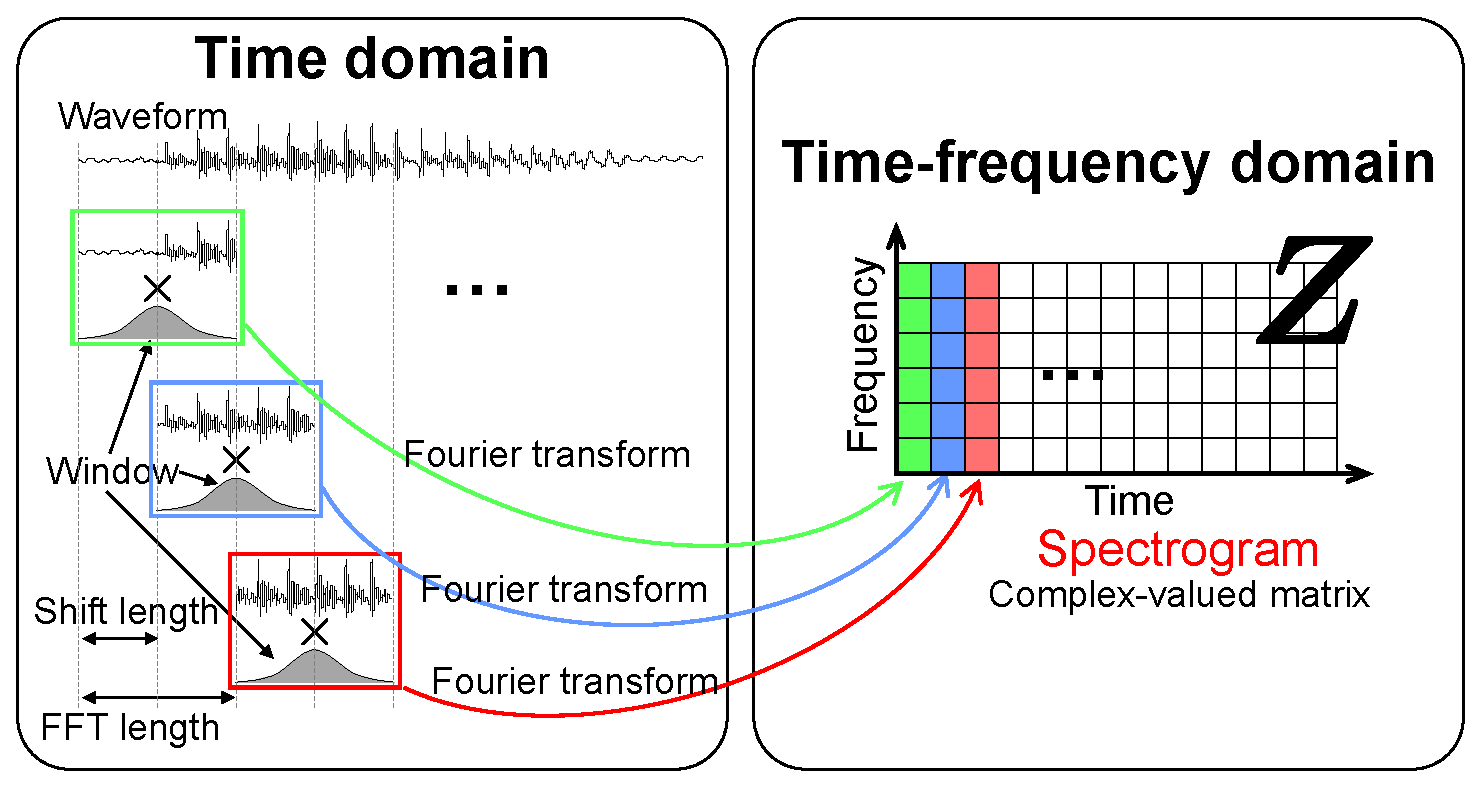
\includegraphics[width=0.95\columnwidth]{figures/stft.eps}
    \end{center}
    \vspace{-8pt}
	\caption{Mechanism of STFT.}
	\label{fig:stft}
\end{figure}
%%%%%%%%%%%%%%%%%%%%%%%%%%%%
STFTはFig.~\ref{fig:stft}に示すような時
間的に変化するスペクトルを表現するための手法である.
STFT の分析窓関数の長さ及びシフト長をそれぞれ$Q$及び$\tau$としたとき,時間領域の信号
$z(l)$の$j$番目の短時間区間(時間フレーム)の信号は次式で表される.
\begin{align}
    \bm{z}^{(j)} &= \left(z\left((j-1)\tau+1\right), z\left((j-1)\tau+2\right), \cdots , z\left((j-1)\tau+Q\right) \right)^{T}\\
    &= \left(
    z^{(j)}(1),z^{(j)}(2),\cdots , z^{(j)}(q), \cdots , z^{(j)}(Q)
    \right)^{T}~\in \mathbb{R}^{Q}
\end{align}
ここで,$j= 1, 2, \cdots , J$及び$q= 1, 2, \cdots , Q$は,それぞれ時間フレーム及び時間フレーム内のサン
プルを示す.また,セグメント数$J$は次式によって与えられる.
\begin{align}
    J = \frac{L}{\tau}
\end{align}
また,各時間フレームの信号のSTFTは次式のようにして求められる.
\begin{align}
\bm{Z}= {\rm STFT}_{\bm{\omega}}(\bm{z})~\in \mathbb{C}^{I \times J}
\end{align}
また,スペクトログラム$\bm{Z}$の$(i, j)$ 番目の要素は次式で表される.
\begin{align}
    z_{ij}= \sum_{q=1}^{Q}\omega(q)z^{(j)}(q){\rm exp}\left\{\frac{-\iota2\pi(q-1)(i-1)}{F}\right\}
\end{align}
ここで$F$は$\lfloor \frac{F}{2}\rfloor+1 =I$を満たす整数($\lfloor \cdot \rfloor$は床関数)を,$i= 1, 2, \cdots , I$は周波数ビンのインデクスを,
$\iota$は虚数単位を,$\bm{\omega}$は分析窓関数を示している.
このように,時間領域の信号は一定幅の短時間ごとに分析窓関数を乗じて離散フーリエ変換を行うことで,横軸が時間,縦軸が周波数のスペクトログラムと呼ばれる複素行列$\bm{Z}$で表すことができる.

%----------------------------------------------
\section{周波数領域におけるBSSの定式化}
\label{sec:formularization}
%----------------------------------------------
今一度,音源数と観測チャネル数(マイクロホン数)をそれぞれ$N$及び$M$とする.
また,各観測音源信号をSTFTすることで得られる,各時間周波数における音声信号,混合信号,及び分離信号をそれぞれ
\begin{align}
  \bm{s}_{ij} &= \left(
	s_{ij,1},s_{ij,2}, \cdots, s_{ij,n}, \cdots, s_{ij,N} 
  \right)^\mathrm{T}~\in \mathbb{C}^{N}\\
  \bm{x}_{ij} &= \left(
      x_{ij,1},x_{ij,2},  \cdots, x_{ij,m}, \cdots  , x_{ij,M} 
  \right)^\mathrm{T}~\in \mathbb{C}^{M} \\
  \bm{z}_{ij} &= \left(
      z_{ij,1},z_{ij,2},  \cdots, z_{ij,n}, \cdots  , z_{ij,N} 
  \right)^\mathrm{T}~\in \mathbb{C}^{N}
\end{align}
と表す.
ここで,$i= 1, 2, \cdots , I$,$j = 1, 2, \cdots , J$,$n = 1, 2, \cdots , N$,及び$m =
1, 2, \cdots , M $はそれぞれ周波数,時間,音源,チャネルのインデクスを示す.
また,複素スペクトログラム行列$\bm{S}_{n} \in \mathbb{C}^{I\times J}$, $\bm{X}_{m} \in \mathbb{C}^{I\times J}$及び$\bm{Z}_{n} \in \mathbb{C}^{I\times J}$の成分をそれぞれ
$s_{i, j, n}$, $x_{i, j, m}$及び$z_{i, j, n}$ と表す.

%----------------------------------------------
\section{FDICA}
\label{sec:fdica}
%----------------------------------------------
\ref{sec:ica}節で説明したように,ICAとは,観測信号が独立信号の線形結合として観測される場合に,各信号間の独立性を最も高めるように線形分離行列を推定することでBSSを実現する手法である.
しかし,実際に観測される音声信号には残響の影響を受けており,線形時不変なインパルス応答が畳み込まれて混合される.
インパルス応答の畳み込みは残響長$R$を用いて次式のように表される.
\begin{align}
  \bm{x}(l) = \sum_n \sum_{l^{'}=0}^{R-1} \tilde{\bm{a}}_n(l^{'}) \bm{s}_n(l-l^{'})
  \label{f:tatami}
\end{align}
ここで,$\tilde{\bm{a}}_n(l)$は,音源$n$に対する畳み込み混合係数ベクトル(音源$n$からマイクロフォン$m$までのインパルス応答をまとめたもの)である.
これを分離するためには逆畳み込みフィルタを推定することが必要となる.
一般的に逆畳み込みフィルタの推定は容易ではないことから,時間領域でのICAによるBSSは困難である.
この問題を解決するために,式(\ref{f:tatami})の時間領域における畳み込み混合を,STFTによって周波数領域上での瞬時混合に変換し,時間周波数領域で周波数毎にICAを行うFDICAが提案された.

FDICAでは,周波数毎の時不変な混合行列 $\bm{A}_{i} = (\bm{a}_{i, 1} ~\bm{a}_{i, 2} ~\cdots ~\bm{a}_{i, n}~\cdots,\bm{a}_{i, N} )\in \mathbb{C}^{M\times N}$を定義し,混合信号が次式で表現できると仮定する.
\begin{align}
 \bm{x}_{ij} = \bm{A}_i\bm{s}_{ij}
\end{align}
この混合モデルは,STFTの窓長が室内残響よりも長い場合にのみ成立する.
以後,決定的な系($M=N$)を仮定すると,混合行列$\bm{A}_{i}$が正則であれば,分離行列$\bm{W}_i=\bm{A}_i^{-1}=(\bm{w}_{i,1}~\bm{w}_{i,2}~ ...~ \bm{w}_{i, n}~ ... ~\bm{w}_{i, N})^{\mathrm{H}}$を用いて,分離信号を次式で表せる.
\begin{align}
 \bm{z}_{ij} = \bm{W}_{i}\bm{x}_{ij} \label{eq:sep}
\end{align}
ここで,$\cdot^\mathrm{H}$はベクトルや行列のエルミート転置を示す.
分離行列の行ベクトルである$\bm{w}_{i,n}\in\mathbb{C}^M$は,周波数$i$において,観測信号から$n$番目のみの音源へ変換する分離フィルタである.
このようにFDICAでは,観測信号$\bm{x}_{ij}$の各周波数ビンに対しそれぞれ独立にICA を適用することで,周波数毎の分離行列$\bm{W}_{i}$を全周波数にわたって推定することで音源分離を行う.

%----------------------------------------------
\section{パーミュテーション問題とその解決}
\label{sec:pp}
%----------------------------------------------
FDICA中で周波数毎に適用しているICAは,音源間の統計的独立性のみに基づいて分離行列を推定するため,分離音源の周波数毎のスケール及び順番に関しては不定である.
従って,FDICAの推定分離行列を$\hat{\bm{W}}_i$とすると,次式のような不定性が残る.
\begin{align}
	\hat{\bm{W}}_{i} &= \bm{D}_{i}\bm{P}_{i}  \bm{W}_{i}
\end{align}
ここで,$\bm{P}_i \in \{0, 1\}^{N \times N}$は分離行列$\bm{W}_{i}$の行ベクトル$\bm{w}_{i, n}$の順番を入れ変えうるパーミュテーション行列(置換行列)である.
$\bm{D}_i \in \mathbb{R}^{N \times N}$は,$\bm{w}_{i,n}$のスケールを変化させる可能性のある対角行列である.
すなわち,FDICAで推定される分離信号
\begin{align}
\bm{y}_{ij} &= \hat{\bm{W}}_i\bm{x}_{ij} \\
&=\left( y_{ij,1},y_{ij,2}, \cdots, y_{ij,n}, \cdots, y_{ij,N} \right)^\mathrm{T}~\in \mathbb{C}^{N} \label{eq:sepSig}
\end{align}
は,推定音源の順番やスケールが周波数毎にばらばらになっている状態である.
このうち,$\bm{D}_i$によって生じるスケールの任意性は,プロジェクションバック法\cite{Matsuoka2001_PB}で復元可能である.
一方で,$\bm{P}_i$によって生じる分離信号の順番の任意性(パーミュテーション)を純粋に復元することは,組み合わせ爆発が発生するため容易ではない.
この問題は,一般的にパーミュテーション問題と呼ばれる.
パーミュテーション問題の概要をFig.~\ref{fig:permu}に示す.
ここで,FDICAで推定される分離信号$\bm{y}_{ij}$の音源毎の複素スペクト
ログラム行列を$\bm{Y}_n \in \mathbb{C}^{I \times J}$で表している.
FDICA直後の$\bm{Y}_n$に注目すると,周波数毎での音源分離は達成できている.
しかし,時間周波数構造全体としては,異なるグループの分離信号が1つの時間周波数構造に混在していることが分かる.
これがパーミュテーション問題であり,ICAの分離信号の順番に関する不定性に起因して発生している.
そのため,FDICAにはポスト処理として,分離された音源の順番を全周波数ビンにわたって正しく並べ直す必要がある.
%%%%%%%%%%%%%%%%%%%%%%%%%%%%
\begin{figure}[t]
    \begin{center}
        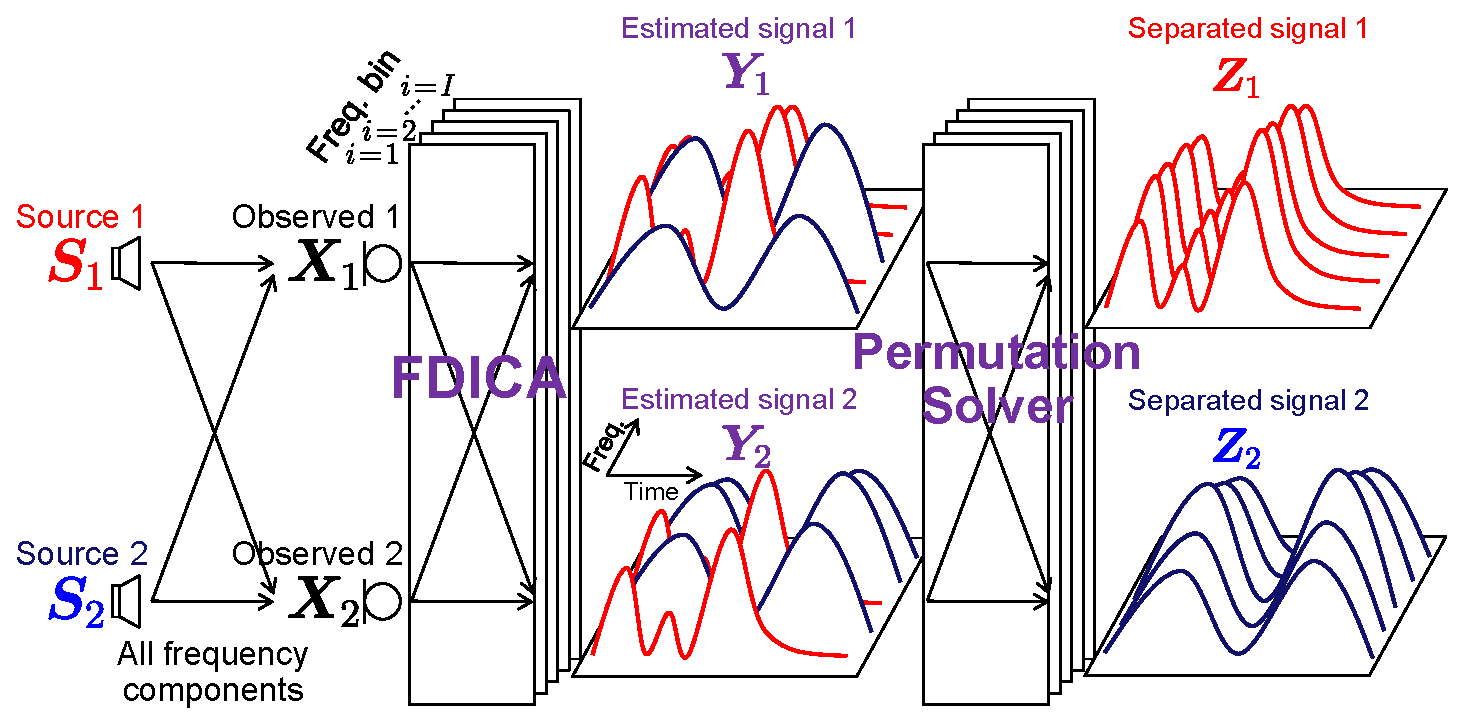
\includegraphics[width=0.95\columnwidth]{figures/permutation_image.eps}
    \end{center}
    \vspace{-8pt}
	\caption{Permutation problem in FDICA, where $N=M=2$.}
	\label{fig:permu}
\end{figure}
%%%%%%%%%%%%%%%%%%%%%%%%%%%%

パーミュテーション問題を解決して得られる分離信号は次式となる.
\begin{align}
\bm{z}_{ij} &= \bm{P}_{i}^{-1}\bm{D}_{i}^{-1}\bm{y}_{ij} \label{eq:z}
\end{align}
%本論文では,この$\bm{P}_{i}^{-1}$を推定することが目的となる.

このパーミュテーション問題を解決するために,これまでにも数々のパーミュテーション解決法が提案されてきた.
代表的な既存手法の1つに,隣接周波数の時系列強度(音源アクティベーション)の相関を用いたパーミュテーション解決法\cite{COR}がある.
これは,分離信号のパーミュテーションが正しければ,隣接した周波数アクティベーション間の相関が高くなりやすいという仮定の下で並べ替える手法である.また,離れた周波数においても,同じ音源のアクティベーション間の相関が高くなるように並び替えられている.
%り,次式のように相関を計算する.
%\begin{align}
%\Tilde{\bm{v}}_{i}(n) &=  \frac{1}{J}\sum_{j=0}^{J} |\bm{y}_{i,j,n}| \\
% {\rm sim}(i) &= \sum_{n\neq m} \frac{\Tilde{\bm{v}}_{i}(n) \cdot \Tilde{\bm{v}}_{i}(m)}{\|
% \Tilde{\bm{v}}_{i}(n)\|~\| \Tilde{\bm{v}}_{i}(m)\|}
%\end{align}
%ここで,$\cdot$は内積を表しており,
他にも,マイクロホンの相対的な位置情報を既知として音源到来方位を計算し,パーミュテーション解決の手掛かりとする手法 \cite{DOA}および両者を組み合わせたパーミュテーション解決法も提案されている.
しかしながら,パーミュテーション問題の解は組み合わせ爆発を起こすことから,上記いずれの手法を用
いても完璧にパーミュテーション問題を解くことは非常に難しく,とくに複数音声の混合信号における高精
度なパーミュテーション問題の解決はいまだできていない.

%----------------------------------------------
\section{深層パーミュテーション解決法}
\label{sec:ivailrma}
%----------------------------------------------

近年では,DNNを用いたパーミュテーション問題解決法が登場している.観測された混合信号$\bm{X}_n$にFDICA適用すると,パーミュテーション問題が生じた分離信号$\bm{Y}_n$が得られる.
これらのパワースペクトログラム$|\bm{Y}_n|^{.2}$から全周波数帯域中の局所的な狭帯域(サブバンド)を定義し,サブバンド毎にデータをDNNに入力し,パーミュテーションを解決する.
サブバンド毎に参照周波数を定義し,その近傍周波数が参照周波数に対して同一音源か否かを判断し,同一音源である場合はDNNの出力として「0」を出力し,同一音源でない場合はDNNの出力として「1」を出力する.2つの周波数これらの推定処理をFig.~に示す.
参照周波数と近傍周波数を($i,i+\omega$),短時間時系列パワー(長さ$\tau $)を以下のように集める.
\begin{align}
  %\bm{d}_{i, \omega, \gamma} &= ({\bm{r}_{i, \gamma, 1}}^\mathrm{T}, {\bm{r}_{i, \gamma, 2}}^\mathrm{T}, {\bm{g}_{i, \omega, \gamma, 1}}^\mathrm{T}, {\bm{g}_{i, \omega, \gamma,2}}^\mathrm{T} )^\mathrm{T}~\in \mathbb{R}_{\geq 0}^{4\tau \times 1},\label{eq:DNNinputVec}\\
  \bm{d}_{i, \omega, \gamma} &= ({\tilde{\bm{r}}_{i, \gamma}}^\mathrm{T}, {\tilde{\bm{g}}_{i, \omega, \gamma}}^\mathrm{T} )^\mathrm{T}~\in \mathbb{R}_{\geq 0}^{4\tau \times 1} \label{eq:DNNinputVec}\\
  \tilde{\bm{r}}_{i,\gamma} &= ({\bm{r}_{i, \gamma, 1}}^\mathrm{T}, {\bm{r}_{i, \gamma, 2}}^\mathrm{T} )^\mathrm{T}~\in \mathbb{R}_{\geq 0}^{2\tau \times 1} \label{eq:DNNinputVecRtilde}\\
  \bm{r}_{i, \gamma, n} &= ( |y_{i, (\gamma-1) \eta+1, n}|^2, |y_{i, (\gamma-1) \eta+2, n} |^2, 
  \cdots, |y_{i, (\gamma-1) \eta+\tau, n}|^2 )^\mathrm{T}~\in \mathbb{R}_{\geq 0}^{\tau \times 1}  \label{tau1}\\
  \tilde{\bm{g}}_{i,\omega,\gamma} &= ({\bm{g}_{i, \omega, \gamma, 1}}^\mathrm{T}, {\bm{g}_{i, \omega, \gamma, 2}}^\mathrm{T} )^\mathrm{T}~\in \mathbb{R}_{\geq 0}^{2\tau \times 1} \label{eq:DNNinputVecGtilde}\\
  \bm{g}_{i,\omega, \gamma, n} &= ( |y_{i+\omega, (\gamma-1) \eta+1, n}|^2, |y_{i+\omega, (\gamma-1) \eta+2, n}|^2,\cdots, |y_{i+\omega, (\gamma-1) \eta+\tau, n}|^2 )^\mathrm{T}~\in \mathbb{R}_{\geq 0}^{\tau \times 1} \label{tau2}
\end{align}
  ここで,行列の $|\cdot|^{.2}$ は,要素ごとの絶対値の二乗を返す.
  また,$\omega=-\Omega, -\Omega+1, \cdots, -1, 0, 1, \cdots, \Omega$は,$\bm{r}_{i,\gamma,n}$と$\bm{g}_{i,\omega,\gamma,n}$の周波数の差であり,$\eta$は,短時間セグメントの時間軸に沿ったストライド幅,$\gamma=1, 2, \cdots, \Gamma$は,短時間セグメントのインデクスである.
  なお,$\Gamma$は,短時間のアクティベーションの長さ$\tau$ とストライド幅$\eta$によって決まる.
  ベクトル $\bm{r}_{i,\gamma,n}$ は,参照周波数$i$の短時間時系列パワーに対応し,ベクトル $\bm{g}_{i,\omega,\gamma,n}$は,Fig.~\ref{fig:input}に示すように,隣接又は局所周波数$i+\omega$ の短時間時系列パワーに対応する.
  DNNの入力ベクトルは,(\ref{eq:DNNinputVec})を正規化したものとして次のようにして表す.
\begin{align}
  \tilde{\bm{d}}_{i, \omega, \gamma} &=\frac{\bm{d}_{i, \omega, \gamma} }{ \|{\bm{d}_{i, \omega, \gamma} }\|_2}~\in \mathbb{R}_{\geq 0}^{4\tau \times 1}  \label{eq:input}
\end{align}
提案するDNNモデルは,0または1を出力する2値分類器である.
推定結果が「0」の場合は,$\bm{r}_{i,\gamma, 1}$と$\bm{g}_{i,\omega,\gamma, 1}$が同一音源であることを意味し,同様に$\bm{r}_{i,\gamma, 2}$と$\bm{g}_{i,\omega,\gamma, 2}$も同一音源である.
一方,推定結果が「1」の場合は$\bm{r}_{i,\gamma, 1}$と$\bm{g}_{i,\omega,\gamma, 1}$(同様に$\bm{r}_{i,\gamma, 2}$と$\bm{g}_{i,\omega,\gamma, 2}$)が異なる音源成分であることを意味している.
これらの推定処理をFig.~\ref{fig:local_dnn}に示す.DNNの予測結果は次のように表せれる.
\begin{align}
  q_{i,\omega,\gamma} = \mathrm{DNN}\left(\tilde{\bm{d}}_{i,\omega,\gamma}\right) \in \{0, 1\}
\end{align}
この結果を時間方向にずらして,全時間フレームに対するDNNの予測処理を走査する.そして,DNNの予測結果を時間軸に対して多数決処理を行うことで,より信頼性の高いサブバンドベクトルを取得する.
サブバンドベクトルは,基準周波数$i$をシフトすることにより全周波数で推定する.ただ,各サブバンドベクトル内の2値は(「0」及び「1」)は異なる意味を持つ可能性がある.これはサブバンド内の周波数成分が.
参照周波数の成分と同一音源か否かを示しているに過ぎず,参照周波数の変化を共に,対応音源が変化する.2音源でサブバンドベクトル内の値が「1」,つまり同一音源ではない場合は,必然的にもう一方の音源となる.ただ,3音源以上になるとサブバンドベクトル内の値が「1」の時,残りのどの音源を一致するのかが判断できない.
そのため,3音源以上になると組み合せ爆発を起こしてしまい,計算量の観点から3音源以上の音源分離は難しい.

%----------------------------------------------
\section{本章のまとめ}
%----------------------------------------------
本章では,提案手法において必要となる基礎理論および各種従来手法について説明した.
次章以降では,より簡潔に精度の良いのBSSを達成するために\ref{sec:fdica}節で導入したFDICAのポスト処理として,DNNに基づくパーミュテーション解決法を新たに提案する.


















%%%%% 第3章 %%%%%
\chapter{結言}
\label{chap:con}

本論文では,FDICAに伴うパーミュテーション問題の解決を目的とし,深層パーミュテーション解決法を新たに提案した.
DNNの入力には,正規化した分離信号から局所時間振幅スペクトログラム成分を抽出した値を用いた.
DNNの出力には,softmax関数を使用し確率値を出力する.この確率値は,各音源の成分である確率を意味する.
DNNの出力である確率値を用いて,推定パーミュテーション行列を作成し分離信号の並び替えを行った.
損失関数にはMSEを用い,推定分離信号と完全分離信号のスペクトログラム間で損失を求め誤差逆伝搬を行った.
テストデータに対してはDNNの入力となる局所時間振幅スペクトログラムをストライド幅に従ってずらしていくことで,時間方向に対して多数決処理を行った.
実験結果より,ブロック単位でのパーミュテーション問題に対しては提案手法を用いて正しく並び替えができることを示した.

最後に今後の展望を述べる.
本論文では,深層パーミュテーション解決手法の可能性に注目しており,基礎的な実験を行ってきた.
本実験では,学習データと検証データの音源に同じスペクトログラムを用いて実験を行っており,未だに音源の時間周波数構造に対する汎化性能は獲得できていない.
この問題を解決するためには,学習データに多数の音声及び音楽信号を用意し,大量のデータをDNNに学習させる必要がある.
また,更なる精度向上のために,DNNの構造としてMLPを用いるのではなく,双方向再帰型DNNを使用することを検討している.
さらには,2音源の実験の拡張版として3音源以上に対する実験も行う必要がある.


%%%%%%%%%%%%%%%%%%%%%%%%%%% 後付 %%%%%%%%%%%%%%%%%%%%%%%%%%%
\backmatter

%%%%% 謝辞 %%%%%
\chapter{謝辞}

本論文は,香川高等専門学校電気情報工学科北村研究室にて行われた研究に基づくものです.

まず,本研究を進めるにあたり,ご多忙のところ熱心に
ご指導くださいました指導教員の北村大地講師に心より感謝申し上げます.
北村大地講師には,論文執筆や研究に関する議論など,細部にわたるまで
丁寧にご指導いただきました.DNNの研究で用いるサーバの増設等にも取り組んでいただき,日々の研究を効率良く行うことができました.心よりありがたくお礼申し上げます.
本論の副査である雛元洋一助教には,論文の構成や記述に関して有益な助言を頂き,大変お世話になりました.ここに厚く御礼申し上げます.
北村研究室の先輩である専攻科2年の岩瀬佑太氏,大藪宗一郎氏,梶谷奈未氏,渡辺瑠伊氏には,音源分離に関する基礎概念のご説明をはじめ,研究の進め方に関して数々のご支援をいただきました.
特に,北村研究室の先輩である専攻科2年の渡辺瑠伊氏には,DNNに関するアドバイスやサーバ管理に関する知見をはじめ,数々のご支援とご助言をいただきました.心より感謝申し上げます.
また,北村研究室同期の川口翔也氏,細谷泰稚氏,村田佳斗氏,溝渕悠朔氏には,日頃のディスカッションのほか,1年に亘る研究室生活を様々な面で支えていただきました.
ここに感謝申し上げます.

最後になりますが,現在に至るまで私の学生生活を金銭的に支え,
暖かく見守って下さった両親には感謝の念に堪えません.
これまで本当にありがとうございました.


%%%%% 参考文献(直接書く場合) %%%%%
\addcontentsline{toc}{chapter}{\bibname} % 参考文献を目次に表示
\begin{thebibliography}{99}
  \bibitem{Kitamura2016taslp}
  D.~Kitamura, N.~Ono, H.~Sawada, H.~Kameoka, and H.~Saruwatari,
  ``Determined blind source separation unifying independent vector analysis and nonnegative matrix factorization,''
  \emph{IEEE/ACM Transactions on Audio, Speech, and Language Processing}, vol. 24, no. 9, pp. 1626--1641, 2016.

  \bibitem{Kitamura2016IWAENC}
  D.~Kitamura, N.~Ono, H.~Saruwatari, Y.~Takahashi, and K. Kondo,
  ``Discriminative and reconstructive basis training for audio source separation with semi-supervised nonnegative matrix factorization,''
  \emph{in Proceedings of International Workshop on Acoustic Signal Enhancement}, 2016, pp. 1--5.
\end{thebibliography}

%%%%% 参考文献(BibTeXを使う場合) %%%%%
% \addcontentsline{toc}{chapter}{\bibname} % 参考文献を目次に表示
% \bibliography{ref_abb_full,references}

%%%%% 発表文献一覧 %%%%%
% {
% \chapter*{発表文献一覧}
% \newcommand{\myname}[1]{\textbf{\underline{#1}}}

% \section*{査読付き国際会議}
% \begin{enumerate}
%   \item \myname{Taro~Kosen} and Daichi~Kitamura,
%     ``Awesome method for surprising something,'' 
%     in Proceedings of \emph{{IEEE} International Conference on Something Awesome}, 
%     2018, pp. 100--103.
%   \item \myname{Taro~Kosen}, Hanako~Kagawa, and Daichi~Kitamura,
%     ``Very awesome method for surprising something,'' 
%     in Proceedings of \emph{{IEEE} International Conference on Something Awesome}, 
%     2019, pp. 100--103.
% \end{enumerate}


% \section*{国内学会}
% \begin{enumerate}
%   \item  \myname{高専太郎}, 北村大地, 
%     ``驚くべき何かの為の素晴らしい手法,''
%     日本何らか学会 2018年春季研究発表会講演論文集, 1-1-10, pp. 100--101, 2018.
%   \item  \myname{高専太郎}, 香川花子, 北村大地, 
%     ``さらに驚くべき何かの為の素晴らしい手法,''
%     日本何らか学会 2019年春季研究発表会講演論文集, 1-1-10, pp. 100--101, 2019.
% \end{enumerate}


% \section*{受賞}
% \begin{enumerate}
%   \item 日本何らか学会 第10回 優秀学生発表賞
% \end{enumerate}
% }


%%%%%%%%%%%%%%%%%%%%%%%%%%% 付録 %%%%%%%%%%%%%%%%%%%%%%%%%%%
\appendix

%%%%% 付録A %%%%%
% \chapter{DNNの人工データに対する予測結果}
% \label{chap:artificial}

% %----------------------------------------------
% \section{接線不等式}
% %----------------------------------------------

% \begin{lemm} \label{lem:aux:sessen} (接線不等式)
% $f(x)$が凹関数であるとき,以下の不等式が成立する.
% \begin{align}
% f(x) \leq f'(\bar{x}) (x - \bar{x}) + f(\bar{x})
% \end{align}
% 不等式中の等号が成立するための条件は$x = \bar{x}$である.
% \end{lemm}

% %----------------------------------------------
% \section{Jensenの不等式}
% %----------------------------------------------

% \begin{lemm} \label{lem:aux:jensen} (Jensenの不等式)
% $\alpha_{i} > 0$を,$\sum_{i} \alpha_{i} = 1$を満たす補助変数とする.
% 関数$f(x)$が凸関数であるとき,$x_{i}\ (i = 1,\ldots,I)$に対して以下の不等式が成立する.
% \begin{align}
% f \left( \sum_{i=1}^{I} \alpha_{i} x_{i} \right) \leq \sum_{i=1}^{I} \alpha_{i} f(x_{i})
% \end{align}
% $f(x)$が狭義凸関数であるとき,不等式中の等号が成立するための条件は
% $x_1 = \cdots = x_i = \cdots = x_I$である.
% \end{lemm}


\end{document}
